


%----------------------------------------------------------------------------------------

\newpage

%\chapter{Thematic Developments}{Développements Thématiques} % Chapter title
\chapter{Développements Thématiques}

\markboth{\thechapter\space Développements Thématiques}{\thechapter\space Développements Thématiques}

\label{app:thematic} % For referencing the chapter elsewhere, use \autoref{ch:name} 

%----------------------------------------------------------------------------------------


Cette annexe regroupe des développements thématiques, c'est à dire qui tombent dans les domaines empiriques, conceptuels et de modélisation. Elles peuvent être relativement éloignées à première vue de nos préoccupations principales, mais sont nécessaires pour la démonstration de points précis.





%----------------------------------------------------------------------------------------


\newpage

%\section[Bridges between Economics and Geography][Ponts entre Géographie et Economie]{Bridges between Economics and Geography : lessons from modeling perspectives}{Ponts entre Géographie et Economie : leçons des perspectives de modélisation}
\section{Bridges between Economics and Geography}{Ponts entre Géographie et Economie}


\label{app:sec:ecogeo}


Cette section rend compte d'une première expérience en ``perspectivisme appliqué'', c'est à dire la tentative de couplage de perspectives sur des objets communs pour créer des ponts entre disciplines. Dans cet esprit, une session spéciale a été organisée, conjointement avec \noun{B. Carantino} (Paris School of Economics) à l'\emph{European Colloqium in Theoretical and Quantitative Geography} pour questionner les liens entre Géographie et Economie. La question de ponts au sein des modèles a été particulièrement étudiée. L'encadré~\ref{frame:app:ecogeo:abstract} ci-dessous présente l'appel à communication.


%%%%%%%%%%%%%
\begin{figure}[h!]
\begin{mdframed}
	
	As Krugman points out, space is for Economic Geography the final frontier, whereas Geographical analyses are somehow far from an advanced integration of economical concepts. What are the existing and potential links? Is there unsurmountable epistemic divergences making bridging approaches irrelevant? For example, the assumptions regarding equilibrium, but also the concepts of equilibrium itself in each discipline may be irreconciliable. This session aims at giving element of answers from a modeling perspective. It is open to case studies of models at the interface and from both disciplines, integrating both elements of spatial analysis and geosimulation together with concepts and methods from economics. It is also open to theoretical or conceptual contributions, in order to bring a broader point of view. An alternative way to study the question is through quantitative epistemology studies, in order to extract empirical endogenous information on the modeling practices themselves. The diversity of views will shed light on potential enrichments on both sides, but also on recurrent difficulties and epistemological divergences, as should illustrate the study of the same objects from totally different perspectives.
	
	\framecaption{}{ECTQG 2017 Special Session : bridges between economics and geography}
\end{mdframed}
\end{figure}
%%%%%%%%%%%%%



\subsection*{Contributions}{Contributions}





\subsection*{Synthesis}{Synthèse des débats}









\stars

\newpage





%----------------------------------------------------------------------------------------


%%%%%%%%%%%
% -- NOT NECESSARY --


%\section{Optimal design of transportation network infrastructure}{Design optimal d'infrastructures de transport}

%\label{app:sec:biological}





%%%%%%%%%%%%%%%%%%%%%%
%\begin{figure}
%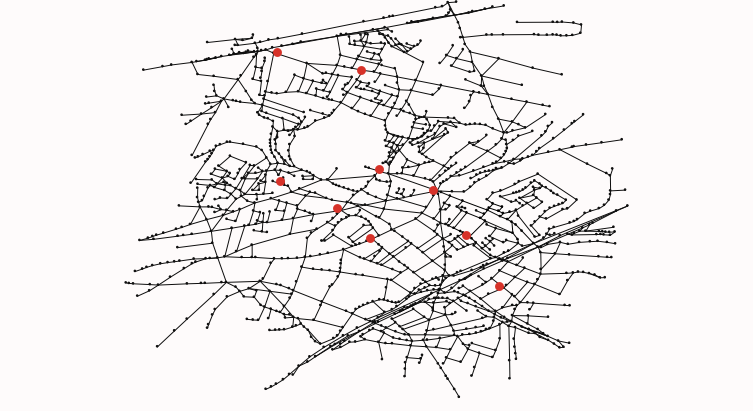
\includegraphics[width=0.45\textwidth]{Figures/NetworkGrowth/tick1}
%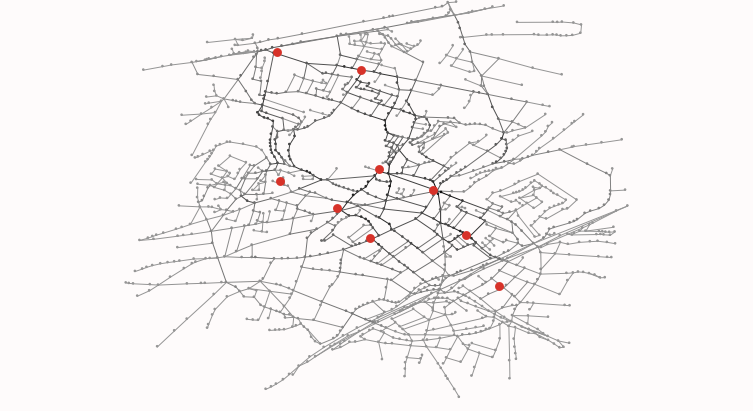
\includegraphics[width=0.45\textwidth]{Figures/NetworkGrowth/tick20}\\
%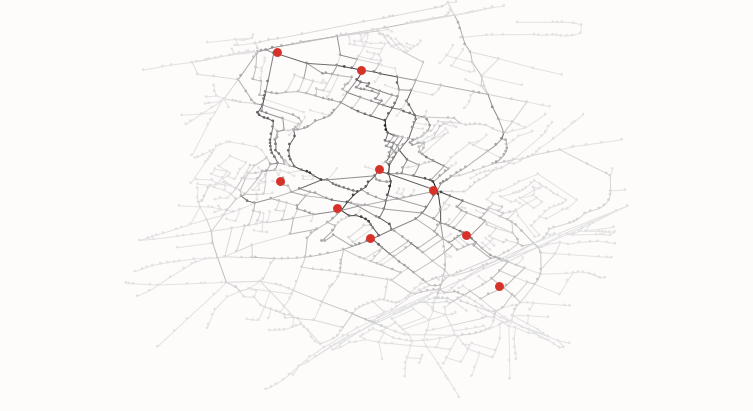
\includegraphics[width=0.45\textwidth]{Figures/NetworkGrowth/tick50}
%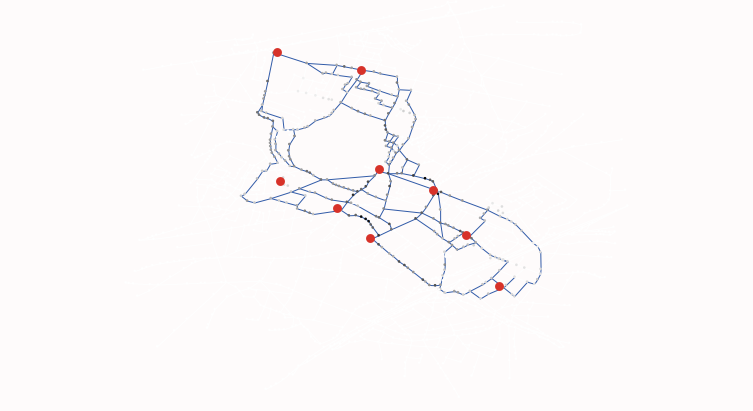
\includegraphics[width=0.45\textwidth]{Figures/NetworkGrowth/reseauFinal}
%\caption[Biological Network Growth][Croissance de réseau biologique]{Example of the application of the slime mould network generation model to the computation of an optimal public transportation network design.}{\comment{(Florent) source ?}}
%\label{fig:slimemould}
%\end{figure}
%%%%%%%%%%%%%%%%%%%%%%%

